\chapter{Vanishing Nodes: correlation between hidden nodes}
\label{why}

In this section, the correlation of hidden-layer neurons is investigated.
If a pair of neurons is highly correlated (for example, the correlation coefficient is equal to $+1$ or $-1$), one of the neurons becomes redundant.
Great similarity between nodes may reduce the effective number of neurons within a network.
In some cases, the correlation of hidden nodes may disable the entire network. This phenomenon is called \textit{Vanishing Nodes}.

% In this section, we would like to show the importance of correlation of hidden layer nodes.
% We will define the correlation metric, show that the highly correlated hidden nodes may reduce the effective width of a neural network, and then connect the width of a network to its representation capability.
% We find that in some cases, the correlation of hidden nodes in a network may disable the whole network.
% We name this phenomena as \textit{vanishing nodes}, and we provide an intuitive example to demonstrate it.

First, consider a deep feed-forward neural network with depth $L$.
For simplicity of analysis, we assume all layers have the same width $N$.
The weight matrix of layer $l$ is $\mathbf{W}_l\in \mathbb{R}^{N\times N}$, the bias of layer $l$ is $\mathbf{b}_l\in \mathbb{R}^N$ (a column vector), and the common activation function of all layers is $\phi(\cdot):\mathbb{R}\rightarrow \mathbb{R}$. The input of the network is $\mathbf{x}_0$, and the nodes at output layer $L$ denote $\mathbf{x}_L$. The pre-activation of layer $l$ is $\mathbf{h}_l\in \mathbb{R}^N$ (a column vector), and the post-activation of layer $l$ is $\mathbf{x}_l\in \mathbb{R}^N$ (a column vector). That is, $\forall l \in \{1, ..., L\}$,

\begin{equation}
    \mathbf{h}_l=\mathbf{W}_l\mathbf{x}_{l-1}+\mathbf{b}_l,\;\;\;
    \mathbf{x}_{l}=\phi(\mathbf{h}_l).
\label{network_eqn}
\end{equation}

The variance of node $i$ is defined as $\sigma_i^2\overset{\Delta}{=}\mathbb{E}_{\mathbf{x}_0}[(x_{l(i)}-\overline{x_{l(i)}})^2]$, and the squared correlation coefficient ($\rho_{ij}^2$) between nodes $i$ and $j$ can be computed as $\rho_{ij}^2\overset{\Delta}{=}
\frac
{\mathbb{E}_{\mathbf{x}_0}[(x_{l(i)}-\overline{x_{l(i)}})(x_{l(j)}-\overline{x_{l(j)}})]^2}
{\mathbb{E}_{\mathbf{x}_0}[(x_{l(i)}-\overline{x_{l(i)}})^2]\mathbb{E}_{\mathbf{x}_0}[(x_{l(j)}-\overline{x_{l(j)}})^2]},$
where $\rho_{ij}^2$ ranges from $0$ to $1$.
Nodes $x_{l(i)}$ and $x_{l(j)}$ are highly correlated only if the magnitude of the correlation coefficient between two nodes $\rho_{ij}$ is nearly 1. $\rho_{ij}^2$ indicates the magnitude of similarity between node $i$ and node $j$.
If $\rho_{ij}$ is close to $+1$ or $-1$, then node $i$ can be approximated in a linear fashion by node $j$. Great similarity indicates redundancy. If nodes of hidden layers exhibit great similarity, the effective number of nodes will be much lower than the original network width. Therefore, we call this phenomena \textit{Vanishing Node Problem}.



%Recent works have put emphasis on the depth of a neural network, since the \textit{width} of a neural network also matters.
%According to the "universal approximation theorem" proved by \cite{universal}, a single hidden layer with a finite number of neurons can approximate continuous functions on compact subsets.
%That is, the number of neurons in a network is closely related to its representation power, which is .

%Vanishing node is a problem that in some cases, several nodes in hidden layers or the output layer in a neural network architecture are highly correlated even if nodes of the input layer are independent.
%Correlations imply dependencies, and dependencies produce redundancy.
%That is, in the worst case, all of hidden nodes or output nodes are so correlated that if we remove the redundant nodes, the number of remaining nodes are much less than the original network width.
%Therefore, we name this phenomena as the \textit{vanishing node problem}.

% \begin{figure}
    \begin{minipage}[c]{0.4\textwidth}
        \caption{We use the product of many Gaussian-initialized matrices as our \textit{"correlated-initialized"} weight matrix. To show the levels of correlation versus the number of matrices in the product, we plot the averaged cosine similarities of weight vectors. Notice that the number of nodes $N$ in hidden layers are all 6.}
        \label{fig:sec3_sim1}
    \end{minipage}\hfill
    \begin{minipage}[c]{0.5\textwidth}
        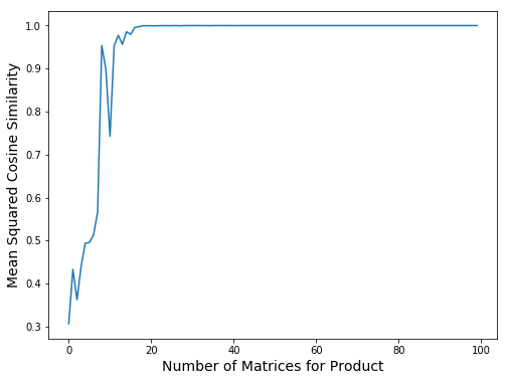
\includegraphics[width=\textwidth]{CorrelatedInitialization}
    \end{minipage}
\end{figure}

%\section{Results} \label{results}

In the following section, we propose a metric to measure the quantitative property of vanishing nodes for a deep feed-forward neural network.
Theoretical analysis of the metric indicates that the quantitative property of vanishing nodes is proportional to the network depth and inversely proportional to the network width.
The quantity is shown analytically to depend on the statistical property of weights and the nonlinear activation function. 

% In this section, we will (1) provide a theoretical analysis on the accumulation of the node correlation just after the weight initialization (2) give a numerical results for presenting that the weights update via back-propagation will intensify the node correlation.

%\section{Network Depth Makes Initial Correlations Accumulate} \label{initial}
\section{Vanishing Node Indicator} \label{initial}

Consider the network architecture defined in \eqref{network_eqn}. In addition, the following assumptions are made: (1) The input $\mathbf{x}_0$ is zero-mean, and the features in $\mathbf{x}_0$ are independent and identically distributed. (2) All weight matrices $\mathbf{W}_l$ in each layer are initialized from the same distribution with variance $\sigma_w^2/N$. (3) All the bias vectors $\mathbf{b}_l$ in each layer are initialized to zero.
% We would like to provide an analysis on the correlation of output nodes in a deep neural network. We will first setup a network, define a metric for measuring the correlation, perform theoretical analysis on the metric, and then provide several results of numerical simulations.

% To analyze the correlation of output layer nodes toward depth, we need to define a metric to measure the output layer node correlation.
% First, consider the network architecture we defined in \eqref{network_eqn}.
% In particular, we have made several assumptions: (1) The input $\mathbf{x}_0$ is zero-mean, and features in $\mathbf{x}_0$ are independent and identically distributed. (2) All the weight matrices $\mathbf{W}_l$ in each layer are initialized from a same distribution with variance $\sigma_w^2/N$. (3) All the bias vectors $\mathbf{b}_l$ in each layer are initialized to zero.

The input-output Jacobian matrix $\mathbf{J}\in\mathbb{R}^{N\times N}$  is defined as the first-order partial derivative of the output layer with respect to the input layer, which can be rewritten as $\frac{\partial\mathbf{x}_L}{\partial\mathbf{x}_0}=\prod_{l=1}^{L}\mathbf{D}_l\mathbf{W}_l$,
where $\mathbf{D}_l\overset{\Delta}{=} diag(\phi'(\mathbf{h}_l))$ is the derivative of point-wise activation function $\phi$ at layer $l$.
% With the input-output Jacobian and the given assumptions, we can perform the first-order forward approximation:
To conduct a similar analysis as \cite{mft:linear}, consider the first-order forward approximation:
$\mathbf{x}_L-\overline{\mathbf{x}_L} \approx \mathbf{Jx}_0$. Therefore, the covariance matrix of the nodes ($\mathbf{C}\in\mathbb{R}^{N\times N}$) at the output layer  can be computed as

\begin{equation}
    \mathbf{C} \overset{\Delta}{=}
    \mathbb{E}_{\mathbf{x}_0}[(\mathbf{x}_L-\overline{\mathbf{x}_L})(\mathbf{x}_L-\overline{\mathbf{x}_L})^T]
    \approx
    \mathbb{E}_{\mathbf{x}_0}[(\mathbf{Jx}_0)(\mathbf{Jx}_0)^T]
    =
    \mathbf{J}\mathbb{E}_{\mathbf{x}_0}[\mathbf{x}_0\mathbf{x}_0^T]\mathbf{J}^T
    =
    \sigma_x^2\mathbf{J}\mathbf{J}^T,
    \label{covariance_eqn}
\end{equation}

where $\sigma_x^2$ is the common variance of features in $\mathbf{x}_0$, and the expected values are calculated with respect to the input $\mathbf{x}_0$. For notational simplicity, we omit the subscript $\mathbf{x}_0$ of the expectations in the following equations. 
It can be easily derived that the squared covariance of nodes $i$ and $j$ is equal to the product of the squared correlation coefficient and the two variances. That is, $[C_{(ij)}]^2=\rho_{ij}^2\sigma_i^2\sigma_j^2$.

In this paper, we propose the \textit{Vanishing Node Indicator (VNI)} $R_{sq}$ to quantitatively characterize the degree of vanishing nodes for a given network architecture. It is defined as follows:

\begin{equation}
    R_{sq}\overset{\Delta}{=}
    \frac{\sum_{i=1}^N\sum_{j=1}^N\rho_{ij}^2\sigma_i^2\sigma_j^2}
{\sum_{i=1}^N\sum_{j=1}^N\sigma_i^2\sigma_j^2}.
\label{rsq_def}
\end{equation}

VNI calculates the weighted average of the squared correlation coefficients $\rho_{ij}^2$ between output layer nodes with non-negative weights $\sigma_i^2\sigma_j^2$. Basically, VNI $R_{sq}$, which ranges from $1/N$ to $1$, summarizes the similarity of the nodes at the output layer. If all nodes are independent of each other, the correlation coefficients $\rho_{ij}$ will be 0 (if $i\neq j$) or 1 (if $i=j$) and $R_{sq}$ will become the minimum value of $1/N$.
Otherwise, if all of the output nodes are highly correlated, then all squared correlation coefficients $\rho_{ij}^2$ will be nearly 1, and therefore $R_{sq}$ will reach the maximum value of $1$.
Note that the weights $\sigma_i^2\sigma_j^2$ in the weighted average can be interpreted as the importance of the output-layer nodes $i$ and $j$. If all of the output layer nodes have equal variances, VNI $R_{sq}$ is simply reduced to the average of the squared correlation coefficients $\rho_{ij}^2$.


\begin{figure}[h]
\centering
\newcommand{\myWidth}{0.48\textwidth}
\begin{subfigure}{\myWidth}
  \centering
  \caption{Network width $N=200$}
  \includegraphics[width=1.0\linewidth,trim={0 0 0 0.8cm},clip]{"MNIST_TanhWidth200(059)"}
  \label{fig:sec4_sim2_a}
\end{subfigure}

\begin{subfigure}{\myWidth}
  \centering
  \caption{Network width $N=500$}
  \includegraphics[width=1.0\linewidth,trim={0 0 0 0.8cm},clip]{"MNIST_TanhWidth500(059)"}
  \label{fig:sec4_sim2_b}
\end{subfigure}%

\caption{
The results of VNI $R_{sq}$ with respect to network depth $L$ for the network width 200 and 500. The red line is calculated from \eqref{rsq_moment}, the blue line is computed from \eqref{rsq_def} with the input data of zero mean and i.i.d input data, and the green line is computed from \eqref{rsq_def} with MNIST data.
%from theoretical analysis (red), simulation with i.i.d. inputs (blue) and simulation with MNIST inputs (green).
The VNI $R_{sq}$ expressed in \eqref{rsq_moment} is very close to the original definition in \eqref{rsq_def}.
% Note that the theoretical value of VNI is $R_{sq}\approx\frac{1}{N}\Big(\frac{L}{0.998}+1\Big)$ for the scaled-Gaussian weight  initialization ($s_1=-1$) and the $Hard\text{-}Tanh$ activation ($\mu_k=erf\big(\frac{1}{\sqrt{2\cdot 0.1}}\big)$).
}
\label{fig:sec4_sim2}
\end{figure}


With the covariance matrix defined in \eqref{covariance_eqn} and the formulas for matrix traces, VNI $R_{sq}$ can be expressed as the formula of the covariance matrix as
\begin{equation}
    \begin{aligned}
    R_{sq}
    &=\frac{
    \sum_{i=1}^N\sum_{j=1}^N\mathbb{E}_{\mathbf{x}_0}
    [(x_{L(i)}-\overline{x_{L(i)}})(x_{L(j)}-\overline{x_{L(j)}})]^2
    }{
    \sum_{i=1}^N\sum_{j=1}^N
    \mathbb{E}_{\mathbf{x}_0}[(x_{L(i)}-\overline{x_{L(i)}})^2]
    \mathbb{E}[(x_{L(j)}-\overline{x_{L(j)}})^2]
    }\\
    &=
    \frac{\sum_{i=1}^N\sum_{j=1}^N[C_{(ij)}]^2}
    {\sum_{i=1}^N\sum_{j=1}^NC_{(ii)}C_{(jj)}}
    =
    \frac{tr(\mathbf{C}{\mathbf{C}}^T)}
    {tr(\mathbf{C})^2}
    ,
    \end{aligned}
    \label{rsq_eqn}
\end{equation}
where $tr(\cdot)$ is the matrix trace operation.

From \eqref{covariance_eqn}, substituting $\sigma_x^2\mathbf{JJ}^T$ for $\mathbf{C}$ in \eqref{rsq_eqn}, and noting that $tr(\mathbf{A}^k)$ is equal to the sum of eigenvalues to the $k$-th power of symmetric matrix $\mathbf{A}$ \cite{matrix}, an approximation of $R_{sq}$ can be obtained:

\begin{equation}
    R_{sq}\approx
    \frac{tr(\mathbf{JJ}^T\mathbf{JJ}^T)}{tr(\mathbf{JJ}^T)^2}
    =\frac{\sum_{k=1}^N\lambda_k^2}{(\sum_{k=1}^N\lambda_k)^2}
    =\frac{N\cdot m_2}{(N\cdot m_1)^2}
    =\frac{m_2}{Nm_1^2},
    \label{rsq_eigen}
\end{equation}

where $\lambda_k$ is the $k$-th eigenvalue of $\mathbf{JJ}^T$, and $m_i$ is the $i$-th moment of eigenvalues of $\mathbf{JJ}^T$.

%In \eqref{rsq_eigen}, we show that  $R_{sq}$ is related to the moments of eigenvalues of $\mathbf{JJ}^T$. Since the moments of eigenvalues of $\mathbf{JJ}^T$ have been analyzed in previous work (\cite{mft:spectral},) we would like to insert the result for the moments of eigenvalues, which is related to the network depth $L$, the network width $N$, the activation function $\phi(\cdot)$ and weight initialization, into the approximation of $R_{sq}$.

%For simplicity, let's assume that the weights of all layers $\mathbf{W}_l$ share a common distribution as $\mathbf{W}$. Also, assume the variances of all hidden layers are the same, which implies the $\mathbf{D}_l$ share a common distribution as $\mathbf{D}$.
%According to the free probability theory described by \cite{mft:spectral}, we consider the expansion of the S-transform  associated with the weights and we define $s_k$ as the $k$-th moment of S-transform. Also, we reuse the definition $\mu_k$ as $\int\mathcal{D}h[\phi'(\sigma_hh)]^{2k}$ where the standard deviation of the pre-activation is defined as $\sigma_h$.
% Since $\mathbf{D}$ is a diagonal matrix, we can rewrite $\mathbf{D}^T\mathbf{D}$ as $\mathbf{D}^2$. 

In \eqref{rsq_eigen}, we show that  $R_{sq}$ is related to the expected moments of the eigenvalues of $\mathbf{JJ}^T$. Because the moments of the eigenvalues of $\mathbf{JJ}^T$ have been analyzed in previous studies \cite{mft:spectral}, we can leverage the recent results  by \cite{mft:spectral}: $m_1=(\sigma_w^2\mu_1)^L$, and $m_2=(\sigma_w^2\mu_1)^{2L}L\big(\frac{\mu_2}{\mu_1^2}+\frac{1}{L}-1-s_1\big)$,
where $\sigma_w^2/N$ is the variance of the initial weight matrices, $s_1$ is the first moment of the series expansion of the S-transform associated with the weight matrices, and $\mu_k$ are the $k$-th moments of series expansion of the moment generating function associated with activation functions.
If we insert the expressions of $m_1$ and $m_2$ into \eqref{rsq_eigen}, we can obtain an approximation of the expected VNI:

\begin{equation}
    R_{sq}\approx \frac{L}{N}\Big(\frac{\mu_2}{\mu_1^2}+\frac{1}{L}-1-s_1\Big)
    =
    \frac{1}{N}+\frac{L}{N}\Big(\frac{\mu_2}{\mu_1^2}-1-s_1\Big)
    ,
    \label{rsq_moment}
\end{equation}

which shows that VNI is determined by the depth $L$, the width $N$, the moments of the activation functions $\mu_k$ and the statistical property of weights $s_1$. 
Because $R_{sq}$ ranges from $1/N$ to $1$, the approximation in \eqref{rsq_moment} is more accurate when $N>>L$.
Moreover, it can be easily seen that the correlation is inversely proportional to the network width $N$, and proportional to the network depth $L$.
% and for most of the network settings, $\mu_2/\mu_1^2-s_1$ is greater than 1, so the correlation is proportional to the network depth $L$.

To evaluate the accuracy of \eqref{rsq_moment} with respect to the original definition in \eqref{rsq_def}, we design the following experiments. A network width, $N\in\{200, 500\}$, is set. The network depth $L$ is adjusted from $10$ to $100$ with the Hard-Tanh activation function.
%and scaled-Gaussian weight initialization. 
One thousand data points with the distribution $\mathbf{x}_0\sim Gaussian(\mu_x=0, \sigma^2_x=0.1)$ and 50,000 training images in MNIST dataset \cite{mnist} are fed into the network.
%as the "i.i.d. inputs" and the "MNIST dataset" respectively.
In each network architecture, the weights are initialized with scaled-Gaussian distribution \cite{xavier} of various random seeds for 100 runs.
The $R_{sq}$ calculated from \eqref{rsq_def} is then recorded to compute the mean and the standard deviation with respect to various network depths $L$.
%and then record the mean and the standard deviation of $R_{sq}$ via \eqref{rsq_def} as the vertical axis.
%The horizontal axis is the network depth $L$. 
The results are shown in Figure \ref{fig:sec4_sim2} as the blue and green lines denoted “Simulation i.i.d. inputs” and "Simulation MNIST dataset." The red line denoted as “Theoretical” is the result calculated from \eqref{rsq_moment}. This experiment demonstrates that VNI expressed in terms of the network parameters in \eqref{rsq_moment} is very close to the original definition in \eqref{rsq_def}.
Similar results are obtained with different activations (e.g., Linear, ReLU) and different weight initialization (e.g., scaled uniform distribution).

Figure \ref{fig:sec4_sim3} plots the squared correlation coefficients between output nodes, which are evaluated with 50,000 training images in the MNIST dataset \cite{mnist} for various network architectures. White indicates no correlation, and black means that $\rho_{ij}^2 = 1$. Figure \ref{fig:sec4_sim3} (a) plots the squared correlation coefficients for four architectures with the same network width ($N=200$) at different depths (5, 50, 300, and 1000). Figure \ref{fig:sec4_sim3} (b) shows the architectures with the same depth ($L=100$) and different widths (5, 50, 200, 1000).  
This shows that the vanishing node phenomenon becomes evident with respect to the depth and inversely proportional to the width.

% In Figure \ref{fig:sec4_sim2}, we set the network width $N\in\{200, 500\}$, adjust the network depth $L=10\sim100$, and then feed 1000 input data points following the distribution $\mathbf{x}^0\sim Gaussian(\mu_x=0, \sigma^2_x=0.1)$.
% In order to observe the correlation related to $L$ and $N$, we run 100 times simulation for every data point, and then record the mean and the standard deviation of $R_{sq}$ via \eqref{rsq_def} as the vertical axis.
% The horizontal axis is network depth $L$.
% We can observe that $R_{sq}$ evaluated from the simulation are quite close to the analytical results in \eqref{rsq_moment}.%, which implies that $R_{sq}$ are proportional to $L$ and inversely proportional to $N$.

% In Figure \ref{fig:sec4_sim3}, we feed the input data $\mathbf{x}^0\sim Gaussian(\mu_x=0, \sigma^2_x=0.1)$ into the specific network as described in the caption. The purpose of this figure is to give a straightforward example for \eqref{rsq_moment}. Therefore, we plot the squared correlation coefficients between output nodes, which are evaluated by \eqref{rho_def} with 1000 input data. It is obvious that the degree of vanishing nodes is proportional to the network depth $L$ and inversely proportional to the network width $N$. 

% \begin{figure}
\centering
\newcommand{\myWidth}{.9\textwidth}
\begin{subfigure}{\myWidth}
  \centering
  \caption{Network width $N=6$}
  \includegraphics[width=1.0\linewidth,trim={0 0 0 0.8cm},clip]{"InitialCorrelation - HardTanhWidth6"}
  \label{fig:sec4_sim1_a}
\end{subfigure}%

\begin{subfigure}{\myWidth}
  \centering
  \caption{Network width $N=50$}
  \includegraphics[width=1.0\linewidth,trim={0 0 0 0.8cm},clip]{"InitialCorrelation - HardTanhWidth50"}
  \label{fig:sec4_sim1_b}
\end{subfigure}%

\begin{subfigure}{\myWidth}
  \centering
  \caption{Network width $N=100$}
  \includegraphics[width=1.0\linewidth,trim={0 0 0 0.8cm},clip]{"InitialCorrelation - HardTanhWidth100"}
  \label{fig:sec4_sim1_c}
\end{subfigure}%

\caption{To show the output layer correlation, we plot the scatter plots with 1000 data points of 6 random sampled output layer nodes of the network with network depth $L=100$, $Hard\text{-}Tanh$ activation and scaled-Gaussian weight initialization. The network width $N=6, 50, 100$ from top to bottom respectively. We can see that correlations are much higher when the network width $N$ is small.}
\label{fig:sec4_sim1}
\end{figure}

% In each simulation, the weight initialization follows the scaled-Gaussian distribution with the activation variance-maintaining property, which was discussed by \cite{xavier, he}.

%\begin{figure}
\centering
\newcommand{\myWidth}{0.8\textwidth}

\begin{subfigure}{\myWidth}
  \centering
  \caption{Network width $N=200$}
  \includegraphics[width=1.0\linewidth]{"mnist_FixN=200"}
  \label{fig:sec4_sim3_a}
\end{subfigure}\hspace{3mm}%
\begin{subfigure}{7mm}
  \centering
  \includegraphics[width=1.0\linewidth]{"colorbar"}
\end{subfigure}%

\begin{subfigure}{\myWidth}
  \centering
  \caption{Network depth $L=100$}
  \includegraphics[width=1.0\linewidth]{"mnist_FixL=100"}
  \label{fig:sec4_sim3_b}
\end{subfigure}\hspace{3mm}%
\begin{subfigure}{7mm}
  \centering
  \includegraphics[width=1.0\linewidth]{"colorbar"}
\end{subfigure}%

\caption{The magnitudes of correlation coefficient $\rho_{ij}$ between output nodes.
The black color means $\rho_{ij}^2=1$ while the white color indicates $\rho_{ij}^2=0$.
The top row shows that the correlation is positive related to the network depth $L$, and the bottom row presents that the correlation is negatively related to the network width $N$. Note that we rearrange the node index to cluster the correlated nodes.}
\label{fig:sec4_sim3}
\end{figure}

\section{Impacts of back-propagation} \label{backprop}

In Section \ref{initial}, we showed that the correlation of a network will increase as the depth $L$ increases; in this section, we exploit the manner in which the back-propagation training process will influence the network correlation by the following experiments. 
%that the correlation of nodes are intensified during a back-propagation training process.

%First, the same architecture defined in \eqref{network_eqn} with $L=100$, $N=500$, tanh activation and scaled Gaussian initialization  are used.  50,000 training images of MNIST dataset (\cite{mnist}) are used with the batch size 100 to with  stochastic gradient descent (SGD) optimization and the batch size set to 100.

\begin{figure}
\centering
\newcommand{\myWidth}{0.8\textwidth}

\begin{subfigure}{\myWidth}
  \centering
  \caption{Network width $N=200$}
  \includegraphics[width=1.0\linewidth]{"mnist_FixN=200"}
  \label{fig:sec4_sim3_a}
\end{subfigure}\hspace{3mm}%
\begin{subfigure}{7mm}
  \centering
  \includegraphics[width=1.0\linewidth]{"colorbar"}
\end{subfigure}%

\begin{subfigure}{\myWidth}
  \centering
  \caption{Network depth $L=100$}
  \includegraphics[width=1.0\linewidth]{"mnist_FixL=100"}
  \label{fig:sec4_sim3_b}
\end{subfigure}\hspace{3mm}%
\begin{subfigure}{7mm}
  \centering
  \includegraphics[width=1.0\linewidth]{"colorbar"}
\end{subfigure}%

\caption{The magnitudes of correlation coefficient $\rho_{ij}$ between output nodes.
The black color means $\rho_{ij}^2=1$ while the white color indicates $\rho_{ij}^2=0$.
The top row shows that the correlation is positive related to the network depth $L$, and the bottom row presents that the correlation is negatively related to the network width $N$. Note that we rearrange the node index to cluster the correlated nodes.}
\label{fig:sec4_sim3}
\end{figure}

First, the same architecture defined in \eqref{network_eqn}, with $L=100$, $N=500$, tanh activation,  and scaled Gaussian initialization \cite{xavier}, is used. The network is then trained on the MNIST dataset \cite{mnist} and optimized with stochastic gradient descent (SGD) with a batch size of 100. The network is trained with three different learning rates for different seeds to initialize the weights for 20 runs. We then record the quartiles of VNI ($R_{sq}$) with respect to the training epochs, as shown in Figure \ref{fig:sec5_sim1}.

%Figure \ref{fig:sec5_sim1} displays the results. 
The boundaries of the colored areas represent the first and third quartiles (i.e., the 25th and 75th percentiles), and the line represents the second quartile (i.e., the median) of $R_{sq}$ over 20 trials.
%The horizontal axis is for the training epoch.
% In Figure \ref{fig:sec5_sim2}, we present the pairwise averaged squared correlation coefficients $\rho_{ij}^2$ via its color. The brighter pixels represent higher correlations.
% Note that in Figure \ref{fig:sec5_sim2_a}, the color of layer 100 is dark because the network width $N=500$ is large, relative to the network depth $L=100$.
It shows that in some cases, VNI increases to 1 during the training process, otherwise VNI grows larger initially, and then decreases to a value which is larger than the initial VNI.
Severe intensification of VNI may occur, as shown by the blue line, which is trained at the learning rate of $10^{-2} $. 
Moreover, we observe that training will become much more difficult due to a lack of network representation capability as VNI $R_{sq}$ approaches 1.
Further discussion is provided in Section \ref{experiments} to investigate the impact of VNI by various training parameters.

\begin{figure}
\centering

\newcommand{\myWidth}{0.98\linewidth}
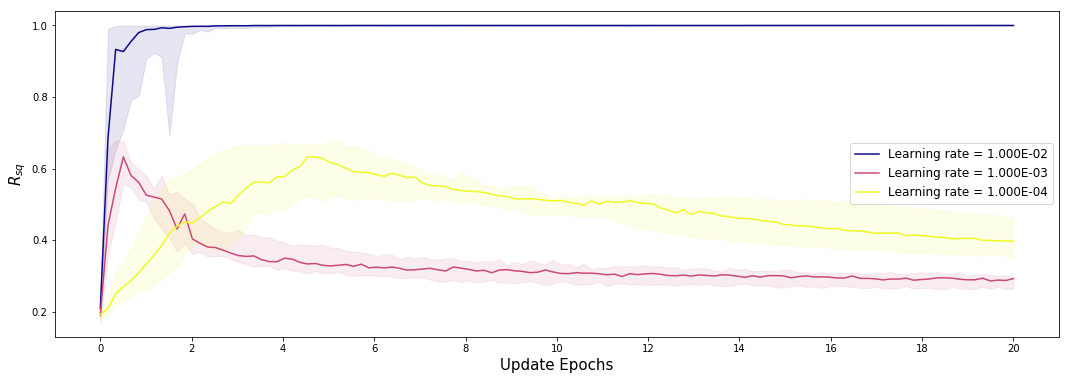
\includegraphics[width=\myWidth]{img/Sec5/sim1/dynamics_e20}
\caption[The dynamics of VNI $R_{sq}$ of the output layer.]
{
The dynamics of VNI $R_{sq}$ of the output layer.
The training is performed on the MNIST dataset 20 times, and then we evaluate the quartiles of the output VNI $R_{sq}$
for different learning rates.
Severe intensification of VNI (increases to 1 ) may occur as shown by the blue line which is trained with the learning rate of $10^{-2}$.
Otherwise VNI rises initially, and then decreases to a value which is larger than the initial VNI.
%It shows that overall, the correlation of each hidden layer is intensified during the back-propagation training. For large learning rate, the output VNI $R_{sq}$ severely increases to 1.
}
\label{fig:sec5_sim1}
\end{figure}


% \begin{figure}
\centering
\newcommand{\myWidth}{0.95\textwidth}
\begin{subfigure}{\myWidth}
  \centering
  \caption{Initial}
  \adjincludegraphics[width=1.0\linewidth,trim={0 0 0 0.8cm},clip]{"Hard-tanh[0]"}
  \label{fig:sec5_sim2_a}
\end{subfigure}%

\begin{subfigure}{\myWidth}
  \centering
  \caption{After 5 updates}
  \adjincludegraphics[width=1.0\linewidth,trim={0 0 0 0.8cm},clip]{"Hard-tanh[5]"}
  \label{fig:sec5_sim2_b}
\end{subfigure}%

\begin{subfigure}{\myWidth}
  \centering
  \caption{After 10 updates}
  \adjincludegraphics[width=1.0\linewidth,trim={0 0 0 0.8cm},clip]{"Hard-tanh[10]"}
  \label{fig:sec5_sim2_c}
\end{subfigure}%
\caption[The averages of squared correlation coefficients $\rho_{ij}^2$ over 50 runs.]
{The averages of squared correlation coefficients $\rho_{ij}^2$ over 50 runs.
It presents that overall, the correlation of each hidden layer are highly intensified.}
\label{fig:sec5_sim2}
\end{figure}


